\section{Graphs}

A \textbf{graph} is a data structure made up of \textbf{nodes} connected by \textbf{pointers}.
Graphs are used to model relationships between entities, such as:
\begin{itemize}
  \item Social networks (one person follows another)
  \item Maps (one city connected to another)
  \item Dependencies (one task must be completed before another)
\end{itemize}

\subsection{Graph Terminology}

In graphs:
\begin{itemize}
  \item Nodes are called \textbf{vertices}
  \item Pointers connecting nodes are called \textbf{edges}
\end{itemize}

Unlike trees and linked lists, graphs have \textbf{no restrictions} on how nodes are connected:
\begin{itemize}
  \item A node can have any number of edges
  \item Cycles are allowed
  \item Nodes don't need to be connected at all
\end{itemize}

The only restriction is the maximum number of edges:
\[
E \leq V^2
\]
This is because every vertex can have an edge pointed to every other vertex \textbf{plus itself}, leading to a maximum of $V^2$ edges. A graph with $V$ vertices and $V^2$ edges is called a \textbf{complete graph}.

\subsection{Directed vs Undirected Graphs}

\textbf{Directed Graph:}
Edges have a direction. An edge from $A$ to $B$ does \textbf{not} imply an edge from $B$ to $A$.

\begin{center}
\begin{tikzpicture}[
  >=Stealth,
  every node/.style={circle, draw, minimum size=10mm},
  edge/.style={->, thick}
]
\node (A) at (0,0) {A};
\node (B) at (3,0) {B};
\node (C) at (1.5,-2) {C};

\draw[edge] (A) -- (B);
\draw[edge] (B) -- (C);
\draw[edge] (C) -- (A);
\end{tikzpicture}

{\small Directed graph: $C \to A$ exists, but $A \to C$ does not}
\end{center}

Trees and linked lists are examples of directed graphs (pointers like \texttt{prev}, \texttt{next}, \texttt{left}, \texttt{right}).

\textbf{Undirected Graph:}
Edges have no direction. If there's an edge between $A$ and $B$, you can traverse in both directions.

\begin{center}
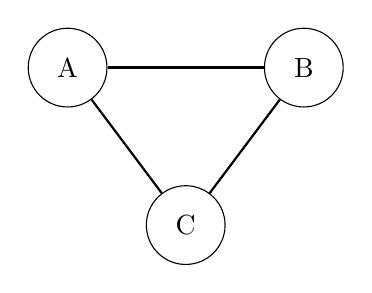
\begin{tikzpicture}[
  every node/.style={circle, draw, minimum size=10mm},
  edge/.style={-, thick}
]
\node (A) at (0,0) {A};
\node (B) at (3,0) {B};
\node (C) at (1.5,-2) {C};

\draw[edge] (A) -- (B);
\draw[edge] (B) -- (C);
\draw[edge] (C) -- (A);
\end{tikzpicture}

{\small Undirected graph: can traverse A--C in both directions}
\end{center}

\subsection{Graph Representations}

Graphs are abstract concepts that can be represented in code using different data structures.

\subsubsection{Matrix (Grid)}

A \textbf{matrix} is a 2D array where:
\begin{itemize}
  \item \texttt{0} represents a free cell (vertex)
  \item \texttt{1} represents a blocked cell
\end{itemize}

\begin{verbatim}
int[][] grid = {{0, 0, 0, 0},
                {1, 1, 0, 0},
                {0, 0, 0, 1},
                {0, 1, 0, 0}};
\end{verbatim}

To traverse the graph, we move \textbf{up, down, left, right} between adjacent 0s. Connected 0s form \textbf{connected components}.

\begin{center}
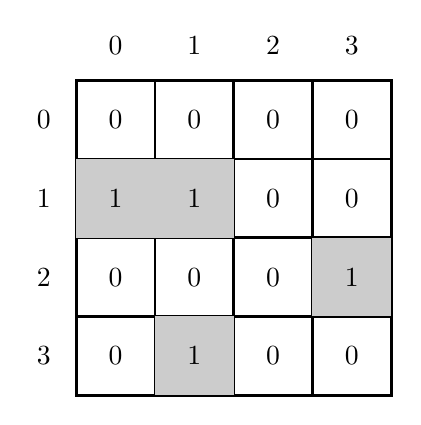
\begin{tikzpicture}[x=1cm,y=1cm]
  \def\cellW{1.0}
  \def\H{1.0}
  
  % Draw grid
  \foreach \row in {0,...,3} {
    \foreach \col in {0,...,3} {
      \draw[line width=1pt] ({\col*\cellW},{-\row*\H}) rectangle ({(\col+1)*\cellW},{(-\row-1)*\H});
    }
  }
  
  % Fill blocked cells (1s)
  \fill[gray!40] ({0*\cellW},{-1*\H}) rectangle ({1*\cellW},{-2*\H}); % [1][0]
  \fill[gray!40] ({1*\cellW},{-1*\H}) rectangle ({2*\cellW},{-2*\H}); % [1][1]
  \fill[gray!40] ({3*\cellW},{-2*\H}) rectangle ({4*\cellW},{-3*\H}); % [2][3]
  \fill[gray!40] ({1*\cellW},{-3*\H}) rectangle ({2*\cellW},{-4*\H}); % [3][1]
  
  % Add values
  \node at ({0.5*\cellW},{-0.5*\H}) {0};
  \node at ({1.5*\cellW},{-0.5*\H}) {0};
  \node at ({2.5*\cellW},{-0.5*\H}) {0};
  \node at ({3.5*\cellW},{-0.5*\H}) {0};
  
  \node at ({0.5*\cellW},{-1.5*\H}) {1};
  \node at ({1.5*\cellW},{-1.5*\H}) {1};
  \node at ({2.5*\cellW},{-1.5*\H}) {0};
  \node at ({3.5*\cellW},{-1.5*\H}) {0};
  
  \node at ({0.5*\cellW},{-2.5*\H}) {0};
  \node at ({1.5*\cellW},{-2.5*\H}) {0};
  \node at ({2.5*\cellW},{-2.5*\H}) {0};
  \node at ({3.5*\cellW},{-2.5*\H}) {1};
  
  \node at ({0.5*\cellW},{-3.5*\H}) {0};
  \node at ({1.5*\cellW},{-3.5*\H}) {1};
  \node at ({2.5*\cellW},{-3.5*\H}) {0};
  \node at ({3.5*\cellW},{-3.5*\H}) {0};
  
  % Row/column labels
  \node[anchor=east] at (-0.2,-0.5) {0};
  \node[anchor=east] at (-0.2,-1.5) {1};
  \node[anchor=east] at (-0.2,-2.5) {2};
  \node[anchor=east] at (-0.2,-3.5) {3};
  
  \node[anchor=south] at (0.5,0.2) {0};
  \node[anchor=south] at (1.5,0.2) {1};
  \node[anchor=south] at (2.5,0.2) {2};
  \node[anchor=south] at (3.5,0.2) {3};
\end{tikzpicture}
\end{center}

\textbf{Space Complexity:} $O(n \cdot m)$ where $n$ is rows and $m$ is columns.

\subsubsection{Adjacency Matrix}

An \textbf{adjacency matrix} is a 2D array where indices represent vertices:
\begin{itemize}
  \item \texttt{adjMatrix[v1][v2] = 1} means an edge exists from \texttt{v1} to \texttt{v2}
  \item \texttt{adjMatrix[v1][v2] = 0} means no edge exists from \texttt{v1} to \texttt{v2}
\end{itemize}

\begin{verbatim}
int[][] adjMatrix = {{0, 0, 0, 0},
                     {1, 1, 0, 0},
                     {0, 0, 0, 1},
                     {0, 1, 0, 0}};
\end{verbatim}

\begin{center}
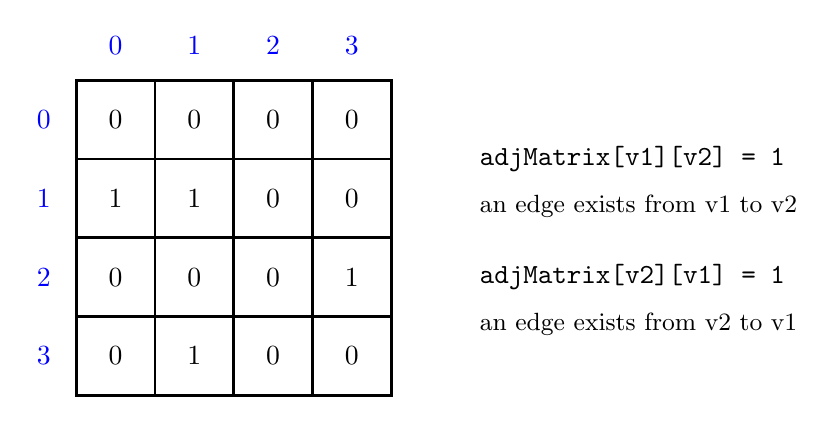
\begin{tikzpicture}[x=1cm,y=1cm]
  \def\cellW{1.0}
  \def\H{1.0}
  
  % Draw grid
  \foreach \row in {0,...,3} {
    \foreach \col in {0,...,3} {
      \draw[line width=1pt] ({\col*\cellW},{-\row*\H}) rectangle ({(\col+1)*\cellW},{(-\row-1)*\H});
    }
  }
  
  % Add values - row 0
  \node at ({0.5*\cellW},{-0.5*\H}) {0};
  \node at ({1.5*\cellW},{-0.5*\H}) {0};
  \node at ({2.5*\cellW},{-0.5*\H}) {0};
  \node at ({3.5*\cellW},{-0.5*\H}) {0};
  
  % Row 1
  \node at ({0.5*\cellW},{-1.5*\H}) {1};
  \node at ({1.5*\cellW},{-1.5*\H}) {1};
  \node at ({2.5*\cellW},{-1.5*\H}) {0};
  \node at ({3.5*\cellW},{-1.5*\H}) {0};
  
  % Row 2
  \node at ({0.5*\cellW},{-2.5*\H}) {0};
  \node at ({1.5*\cellW},{-2.5*\H}) {0};
  \node at ({2.5*\cellW},{-2.5*\H}) {0};
  \node at ({3.5*\cellW},{-2.5*\H}) {1};
  
  % Row 3
  \node at ({0.5*\cellW},{-3.5*\H}) {0};
  \node at ({1.5*\cellW},{-3.5*\H}) {1};
  \node at ({2.5*\cellW},{-3.5*\H}) {0};
  \node at ({3.5*\cellW},{-3.5*\H}) {0};
  
  % Row/column labels
  \node[anchor=east,blue] at (-0.2,-0.5) {0};
  \node[anchor=east,blue] at (-0.2,-1.5) {1};
  \node[anchor=east,blue] at (-0.2,-2.5) {2};
  \node[anchor=east,blue] at (-0.2,-3.5) {3};
  
  \node[anchor=south,blue] at (0.5,0.2) {0};
  \node[anchor=south,blue] at (1.5,0.2) {1};
  \node[anchor=south,blue] at (2.5,0.2) {2};
  \node[anchor=south,blue] at (3.5,0.2) {3};
  
  % Annotations
  \node[anchor=west] at (5,-1) {\texttt{adjMatrix[v1][v2] = 1}};
  \node[anchor=west] at (5,-1.6) {\small an edge exists from v1 to v2};
  
  \node[anchor=west] at (5,-2.5) {\texttt{adjMatrix[v2][v1] = 1}};
  \node[anchor=west] at (5,-3.1) {\small an edge exists from v2 to v1};
\end{tikzpicture}
\end{center}

From the matrix above:
\begin{itemize}
  \item \texttt{adjMatrix[1][0] = 1}: edge from vertex 1 to vertex 0
  \item \texttt{adjMatrix[1][1] = 1}: edge from vertex 1 to itself (self-loop)
  \item \texttt{adjMatrix[2][3] = 1}: edge from vertex 2 to vertex 3
  \item \texttt{adjMatrix[3][1] = 1}: edge from vertex 3 to vertex 1
\end{itemize}

\begin{center}
\begin{tikzpicture}[
  >=Stealth,
  every node/.style={circle, draw, minimum size=10mm},
  edge/.style={->, thick}
]
\node (0) at (0,0) {0};
\node (1) at (3,0) {1};
\node (2) at (3,-3) {2};
\node (3) at (0,-3) {3};

\draw[edge] (1) -- (0);
\draw[edge] (1) to [out=45,in=135,looseness=5] (1); % self-loop
\draw[edge] (2) -- (3);
\draw[edge] (3) -- (1);
\end{tikzpicture}

{\small Graph represented by the adjacency matrix}
\end{center}

\textbf{Drawback:} If the graph has few edges, most of the matrix is wasted storing 0s.

\textbf{Space Complexity:} $O(V^2)$ where $V$ is the number of vertices.

\subsubsection{Adjacency List}

An \textbf{adjacency list} stores only the edges that exist. Each vertex maintains a list of its neighbors.

\begin{verbatim}
class GraphNode {
    int val;
    List<GraphNode> neighbors;

    GraphNode(int val) {
        this.val = val;
        this.neighbors = new ArrayList<>();
    }
}
\end{verbatim}

\begin{center}
\begin{tikzpicture}[x=1cm,y=1cm,>=Stealth]
  % Node boxes
  \foreach \i/\val/\neighbors in {0/0/{}, 1/1/{0}, 2/2/{3}, 3/3/{1}} {
    % Node value box
    \draw[line width=1pt] (0,{-\i*1.2}) rectangle (1,{-\i*1.2-0.8});
    \node at (0.5,{-\i*1.2-0.4}) {\val};
    
    % Arrow to neighbors
    \draw[->,thick] (1,{-\i*1.2-0.4}) -- (1.5,{-\i*1.2-0.4});
  }
  
  % Neighbor lists
  \node[anchor=west] at (1.6,-0.4) {[ ]};
  \node[anchor=west] at (1.6,-1.6) {[0]};
  \node[anchor=west] at (1.6,-2.8) {[3]};
  \node[anchor=west] at (1.6,-4.0) {[1]};
  
  % Labels
  \node[anchor=east] at (-0.2,-0.4) {vertex 0:};
  \node[anchor=east] at (-0.2,-1.6) {vertex 1:};
  \node[anchor=east] at (-0.2,-2.8) {vertex 2:};
  \node[anchor=east] at (-0.2,-4.0) {vertex 3:};
\end{tikzpicture}
\end{center}

Alternatively, using a HashMap:
\begin{verbatim}
Map<Integer, List<Integer>> adjList = new HashMap<>();
adjList.put(0, new ArrayList<>());
adjList.put(1, Arrays.asList(0));
adjList.put(2, Arrays.asList(3));
adjList.put(3, Arrays.asList(1));
\end{verbatim}

\textbf{Advantage:} More space-efficient than adjacency matrix when the graph has few edges.

\textbf{Space Complexity:} $O(V + E)$ where $V$ is vertices and $E$ is edges.

\subsection{Comparison of Representations}

\begin{center}
\begin{tabular}{l c c}
\toprule
\textbf{Representation} & \textbf{Space} & \textbf{Best For} \\
\midrule
Matrix (Grid) & $O(n \cdot m)$ & Grid-based traversal \\
Adjacency Matrix & $O(V^2)$ & Dense graphs (many edges) \\
Adjacency List & $O(V + E)$ & Sparse graphs (few edges) \\
\bottomrule
\end{tabular}
\end{center}